\documentclass{article}

% if you need to pass options to natbib, use, e.g.:
%     \PassOptionsToPackage{numbers, compress}{natbib}
% before loading neurips_2021

% ready for submission
\usepackage[preprint]{neurips_2021}

% to compile a preprint version, e.g., for submission to arXiv, add add the
% [preprint] option:
%     \usepackage[preprint]{neurips_2021}

% to compile a camera-ready version, add the [final] option, e.g.:
%     \usepackage[final]{neurips_2021}

% to avoid loading the natbib package, add option nonatbib:
%    \usepackage[nonatbib]{neurips_2021}

\usepackage[utf8]{inputenc} % allow utf-8 input
\usepackage[T1]{fontenc}    % use 8-bit T1 fonts
\usepackage{hyperref}       % hyperlinks
\usepackage{url}            % simple URL typesetting
\usepackage{booktabs}       % professional-quality tables
\usepackage{amsfonts}       % blackboard math symbols
\usepackage{nicefrac}       % compact symbols for 1/2, etc.
\usepackage{microtype}      % microtypography
\usepackage{xcolor}         % colors
\usepackage{graphicx}       % for figs
\usepackage{amsmath}

\graphicspath{ {../figs/} }  % setting figure path
\bibliographystyle{abbrvnat}

\title{Exploring the development of spotify audio features over time}

\author{%
  Leander Zimmermann\\
  Matrikelnummer 4165446\\
  \texttt{leander.zimmermann@student.uni-tuebingen.de} \\
}

\begin{document}

\maketitle

\begin{abstract}
  This is a test of basic citations \citet{dataset}.
\end{abstract}

\section{Introduction}

Music is a very complicated concept and it is hard to grasp, what makes a person like certain arrangements of sounds and dislike others. Nevertheless it is undeniable, that there is a general trend, which kinds of music tend to be popular. Interestingly this trend seems to change over time, with new genres developing and old styles of music diminishing in popularity.

This report will try to make a connection between basic features of songs and the time they were released. To achieve that we will build regression models to predict the release year from said features and then look at the relationship used by the predictor to get a sense of which features were prominent in which periods of time.

\section{Background}
\subsection{Spotify Audio Features}\label{sec:features}
The features of the songs analysed in the report are generated by spotify.
\citep{spotify_audio_features} \answerTODO{explanation of features}

\subsection{Linear Regression}\label{sec:lin_reg}
Linear regression is a way to fit a function, onto some given data. In our case the inputs of the function are the features mentioned in section~\ref{sec:features} and the desired output is the release year of the song.
Equation~\ref{eq:lin_reg} shows the simplicity of this formula, with the feature vector $x$, the weights $w$, and the target (here the year) $t$.
\begin{align}
  t = w_0 + x_1w_1 + x_2w_2 + \dots + x_nw_n \label{eq:lin_reg}
\end{align}
When the relationship between features and target is more complicated than linear, one can augment this function by introducing a more complicated feature vector. The regression function with a polynomial feature vector is shown in equation~\ref{eq:lin_poly}.
\begin{align}
  t = w_0 + x_1w_{1} + x_1^2w_{2} + x_1x_2w_{3} + \dots + x_nw_{n,1} + x_n^2w_{n,2} \label{eq:lin_poly}
\end{align}
\answerTODO{How w is found}

\subsection{Logistic Regression}\label{sec:log_reg}
Logistic Regression is very similar to Linear Regression. However it is a bit more complicated. The function we seek here, is no longer supposed to output a single number, but rather the probability of some amount of discrete events.

\answerTODO mention sigmoid, vector output, weight matrix and equation~\ref{eq:log_reg}
\begin{align}
  \mathbf{t}_i &= \sigma\Big(W_{i0} + x_1W_{i1}+ x_2W_{i2}+ \dots + x_nW_{in}\Big) \label{eq:log_reg} \\
  \sigma(z) &= \frac{1}{1+e^{-z}}
\end{align}

\section{Methodology}
This section describes how the predictor was build and how this lead to the final result of the report. It was achieved with he use of pandas \citep{pandas} and scikit-learn \citep{sklearn}.

\subsection{Dataset}\label{sec:dataset}
\answerTODO mention how complicated and hoard to predict - also rewrite
The dataset, created by \citet{dataset} is a collection of ca. 1.2 million data points, each representing a song from spotify. For each song it includes the title, album, artist and the corresponding ids. More importantly, it also contains the release year and the spotify audio features, explained in section~\ref{sec:features}. A first look at the data reveals, that the dataset is lopsided when viewed by year.

In order to build a predictor, that is capable of generating an accurate year from the features, all years in question have to entail a certain amount of data points. Therefore we decided to eject all years prior to 1990. This way we are left with 31 years (1990-2020) of data, which contain more than 95\% of the dataset.

\subsection{Preprocessing}

For validation of the predictor, the dataset is divided into a train- and a test-set, in a fairly standard 80-20 split. With that a validation of the resulting coefficients is possible.
To ensure comparable coefficients, the data was then centered to 0 and scaled to unit variance. 
\answerTODO specify features used

\subsection{Predicting the year}

To predict the year from the selected spotify features, we build a linear regression model and (see section~\ref{sec:lin_reg}). Because the relationship between the features and the release year is way more complicated than a linear function could capture, the model was fit on a polynomial feature vector of degree 3.

\subsection{Examination of the linear relationship}

As mentioned above, the actual relationship between the features and the release year is not linear. However, for the purpose of finding out, what features are more or less likely to be high in 
However that does not mean, that there is no linear correlation. To show that this is the case, another linear regression model was fit on on the original (linear) feature vector.






The logistic regression process provides us with a number of coefficients, that tell us how prevalent the predictor estimated a certain feature in a given time span. In other words, when the coefficient of time span $A$ and feature $B$ is high, then feature $B$ is likely to be high for any song, placed in time span $A$ by the predictor.


\section{Results}
\begin{figure}[t]
  \centering
  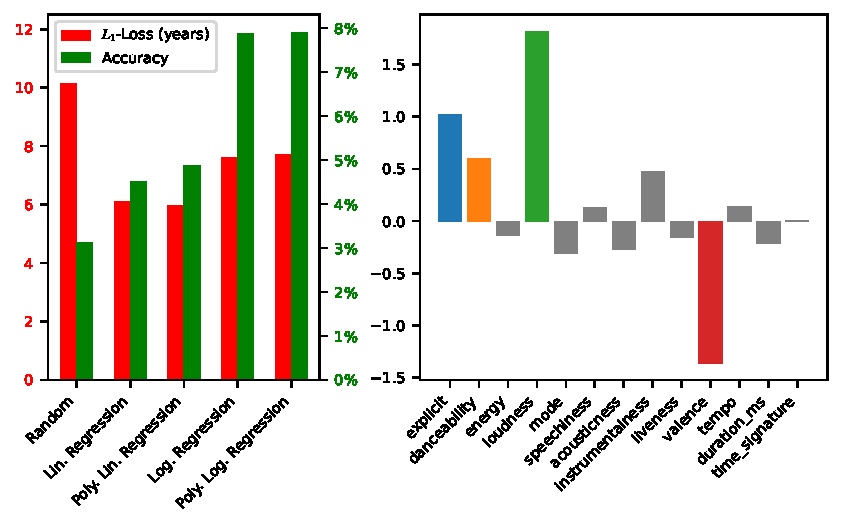
\includegraphics{losses_lincoefs}
  \caption{\emph{Unfair} comparison of the $L_2$-Loss, i.e.  the mean absolute distance in years (lower is better) and accuracies (higher is better) of the Predictors (left) and the coefficients of the linear regression model (right). The accuracies of the linear regression models were calculated by rounding the output values to the nearest full year.}
  \label{fig:losses_lincoefs}
\end{figure}

\begin{figure}[t]
  \centering
  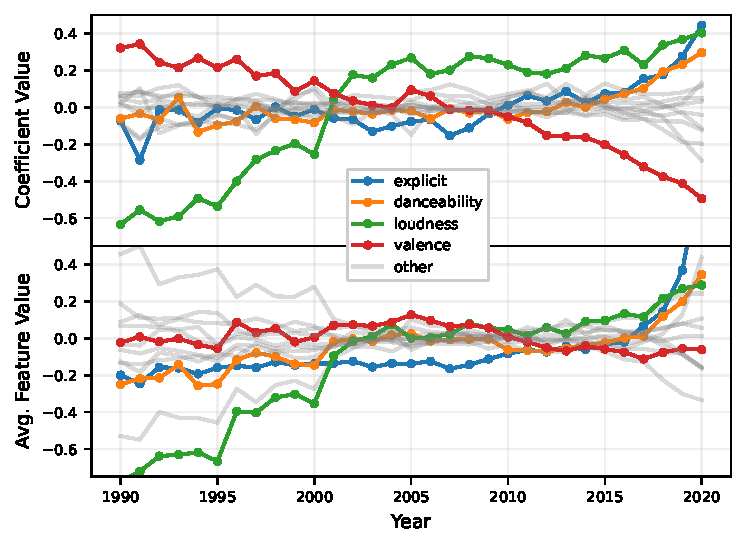
\includegraphics{coefs_avg}
  \caption{The coefficient for each year produced by the logistic regression model (top) and the average value of the features in each year (bottom). The colored lines represent the coefficients with the highest values in many years and their corresponding features. This makes them more important for the logistic regression predictor than the remaining features (grey).} 
  \label{fig:coefs_avg}
\end{figure}
\subsection{Predictions}

The left side of Figure~\ref{fig:losses_lincoefs} shows some evaluation metrics of the models, performed on the test set. 
Both of these comparisons are hardly fair, as the models are optimized on very different things, but the comparison to randomly generated numbers shows us, that none of them are particularly good. Considering the complicated nature of the data, however, this is not very surprising, as mentioned in Section~\ref{sec:dataset}.
Another thing that is clearly visible, is that the linear regression model with polynomial features does not perform significantly better than the simple linear model.

\subsection{Coefficients}

We now try to interpret the coefficients of the models we have build. Because it is much more complicated, while not providing significantly better performance, we throw out the polynomial feature vector. Looking at the coefficients of the linear regression model can already tell us some things about the development of the corresponding features over time. Figure~\ref{fig:losses_lincoefs} shows these coefficients. For example we can now say, that a higher value of the feature \emph{"loudness"} results in a higher output of the model. Thus, in reverse this means that the model assumes songs that have been released later to have a higher \emph{"loudness"}-value.

The logistic regression model gives us a coefficient for each feature in every year, as the output of the model is now a vector of probabilities for the song being released in each year (or alternatively simply the year with the highest probability). These coefficients can be seen in the top part of Figure~\ref{fig:coefs_avg}. While the relationship is not linear, a high coefficient still means a high probability given a high feature value. By looking at this plot, we could for example interpret that, according to the model, in the early 90s many songs have a high valence (i.e. sound happier), while recently more songs with a low valence were released.
Most of the coefficients are very close to 0 in all years and only a few, which can be assumed to have high predictive value, have high and low values in different years. 
In contrast to that, the mean value per year of the features, displayed in the bottom of Figure~\ref{fig:coefs_avg}, does not show the same features with high predictive values standing out at all. Additionally, some curves, like the \emph{valence} coefficient show trends, that the mean does not.

\section{Conclusion}

From the resulting coefficients, one could make the conclusion that in the 90s many songs were relatively happy and quiet, while in the late 2010s the music is much sadder, louder with more songs being rated explicit. While this may or may not be true, experiment conducted here does not support assumptions like that.v Between the arbitrary features the dataset that we know very little about, and the predictions of the models not being very good. We can not confidently conclude anything about the development of music.

\bibliography{references} 

\end{document}
